\chapter{Evaluation}
Evaluation with quantum ripple carry adder~\cite{CDKM04}
\begin{itemize}
    \item What does to quantum ripple carry adder do?
    \item Adds quantum register $a$ to register $b$
    \item usual result for classical values, $a = \ket{1}$ $b = \ket{2}$ result in $\ket{3}$
    \item values in superposition result in results in superposition, $a = \ket{3} + \ket{3}$, $b = \ket{2}$ result in $\ket{3}$
    \item How is it implemented in QASM and Luie
    \item What are the differences?
\end{itemize}

\begin{figure}[htp]
    \centering     
    \lstinputlisting[style=QASM]{../figures/code/evaluation/adder.qasm}
    \caption{CAPTION HERE}
    \label{fig:eval_adder_qasm}
\end{figure}

\begin{figure}[htp]
    \centering     
    \lstinputlisting[style=Luie]{../figures/code/evaluation/adder.luie}
    \caption{CAPTION HERE}
    \label{fig:eval_adder_luie}
\end{figure}

\begin{itemize}
    \item (Possibly compiled qasm in appendix)
    \item Quantum Circuit of algorithm  
\end{itemize}

\begin{figure}[htp]
    \centering     
    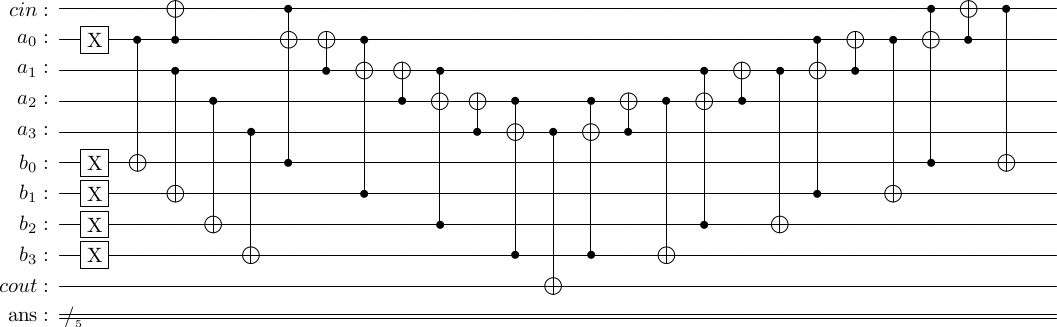
\includegraphics[width=\textwidth]{../figures/images/adderCircuit.png}
    \caption{CAPTION HERE}
    \label{fig:eval_adder_circuit}
\end{figure}

\begin{itemize}
    \item What optimizations can be applied
    \item Circuit after optimizations
    \item Which are applied by default optimizations of quiskit of transpilation? -> none
    \item Why? -> no default peeping control rule
    \item What much is optimized
    \item Depends on input
    \item For only classical, all redundant operations are removed
    \item For input in superposition, optimization effectiveness depends on ``how entangle data''
\end{itemize}

\begin{itemize}
    \item Time taken for compilation, depending on different sizes of registers
    \item Time take for the different optimizations (with different register sizes)
    \item Estimate complexity of optimization, compare to actual runtime
\end{itemize}
